\documentclass{article}
% Adjust the relative path to point to the latex-templates directory

% content/resources/templates/preamble.tex
\usepackage[margin=0.6in]{geometry}
\author{Milav Dabgar}
\usepackage{amsmath,amssymb,amsthm}
\usepackage{booktabs}
\usepackage{multirow}
\usepackage{xcolor}
\usepackage{tcolorbox}
\tcbuselibrary{breakable,skins}
\usepackage[colorlinks=true,linkcolor=blue]{hyperref}
\usepackage{titlesec}
\usepackage{enumitem}
\usepackage{tikz}
\usepackage{pgfplots}
\usepackage{circuitikz}
\usepackage[version=4]{mhchem}
\usepackage{longtable}
\usepackage{array}
\usepackage{float}
\usepackage{caption}
\usepackage{listings}

\lstset{
  basicstyle=\small\ttfamily,
  breaklines=true,
  breakatwhitespace=false,
  postbreak=\mbox{\textcolor{red}{$\hookrightarrow$}\space},
  float=false,
  numbers=left,
  numberstyle=\tiny\color{gray},
  numbersep=10pt,
  xleftmargin=2em,
  keywordstyle=\color{blue},
  commentstyle=\color{green!60!black},
  stringstyle=\color{purple},
  backgroundcolor=\color{gray!5},
  showstringspaces=false,
  tabsize=2,
  captionpos=b,
  keepspaces=true,
  columns=flexible
}

\pgfplotsset{compat=1.18}
\usetikzlibrary{shapes,arrows,positioning,calc,patterns,decorations.pathmorphing,decorations.markings,arrows.meta}

% Color scheme
\definecolor{headcolor}{RGB}{0,102,204}
\definecolor{keycolor}{RGB}{220,20,60}
\definecolor{solutioncolor}{RGB}{34,139,34}
\definecolor{mnemoniccolor}{RGB}{148,0,211}
\definecolor{codecolor}{RGB}{0,0,100}

% Spacing
\setlength{\parskip}{3pt}
\setlist[itemize]{nosep}
\setlist[enumerate]{nosep}

% Title formatting
\titleformat{\section}{\Large\bfseries\color{headcolor}}{\thesection}{1em}{}
\titleformat{\subsection}{\large\bfseries\color{headcolor}}{\thesubsection}{1em}{}

% Pandoc tightlist compatibility
\providecommand{\tightlist}{%
  \setlength{\itemsep}{0pt}\setlength{\parskip}{0pt}}

% Pandoc longtable compatibility
\newcounter{none}
\def\thenone{}


% content/resources/templates/english-boxes.tex

% Custom environments
\newtcolorbox{solutionbox}{
 breakable,
 enhanced,
 colback=solutioncolor!5!white,
 colframe=solutioncolor!75!black,
 fonttitle=\bfseries,
 title=Solution
}

\newtcolorbox{solutionboxnobreak}{
 colback=solutioncolor!5!white,
 colframe=solutioncolor!75!black,
 fonttitle=\bfseries,
 title=Solution
}

\newtcolorbox{keyformula}{
 breakable,
 enhanced,
 colback=keycolor!5!white,
 colframe=keycolor!75!black,
 fonttitle=\bfseries,
 title=Key Formula
}

\newtcolorbox{mnemonicboxenv}{
 breakable,
 enhanced,
 colback=mnemoniccolor!5!white,
 colframe=mnemoniccolor!75!black,
 fonttitle=\bfseries,
 title=Mnemonic
}

\newcommand{\mnemonicbox}[1]{%
  \begin{mnemonicboxenv}
    #1
  \end{mnemonicboxenv}
}


% Custom commands for GTU solutions
% This file defines semantic commands for consistent formatting

% Question command with automatic formatting
\newcommand{\question}[2]{%
  \section*{Question #1}%
  \textbf{#2}%
}

% OR question variant
\newcommand{\questionor}[2]{%
  \section*{Question #1 OR}%
  \textbf{#2}%
}

% Proper table environment with caption
\newenvironment{answertable}[1]{%
  \begin{table}[htbp]
  \centering
  \caption{#1}
}{%
  \end{table}
}

% Proper figure environment for diagrams
\newenvironment{answerdiagram}[1]{%
  \begin{figure}[htbp]
  \centering
  \caption{#1}
}{%
  \end{figure}
}

% Semantic markup for key terms
\newcommand{\keyword}[1]{\textbf{#1}}
\newcommand{\code}[1]{\texttt{#1}}
\newcommand{\classname}[1]{\texttt{#1}}
\newcommand{\methodname}[1]{\texttt{#1}}

% Proper quotation marks
\newcommand{\mnemonic}[1]{``#1''}


\title{Fundamentals of Electronics (DI01000051) - Summer 2025 Solution}
\date{June 12, 2025}

\begin{document}
\maketitle

% ==================================================================
% Q.1
% ==================================================================

\questionmarks{1(a)}{3}{Draw Bi-stable multivibrator using 555 timer IC.}

\begin{solutionbox}
A Bi-stable multivibrator has two stable states (HIGH and LOW). It stays in one state until triggered to switch to the other.

\textbf{Circuit Diagram:}

\begin{center}
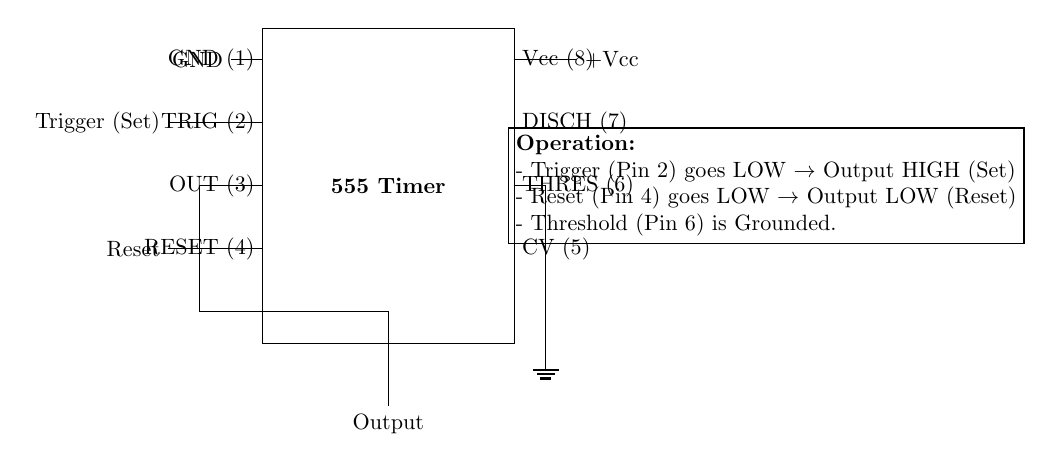
\begin{tikzpicture}[scale=0.8, transform shape]
    % 555 Timer IC
    \draw (0,0) rectangle (4,5);
    \node at (2,2.5) {\textbf{555 Timer}};
    
    % Pins
    \node[left] at (0,4.5) {GND (1)};
    \node[left] at (0,3.5) {TRIG (2)};
    \node[left] at (0,2.5) {OUT (3)};
    \node[left] at (0,1.5) {RESET (4)};
    
    \node[right] at (4,4.5) {Vcc (8)};
    \node[right] at (4,3.5) {DISCH (7)};
    \node[right] at (4,2.5) {THRES (6)};
    \node[right] at (4,1.5) {CV (5)};
    
    % Bi-stable Connections
    % Trigger input (Set)
    \draw (0,3.5) -- (-1.5,3.5) node[left] {Trigger (Set)};
    
    % Reset input (Reset)
    \draw (0,1.5) -- (-1.5,1.5) node[left] {Reset};
    
    % Output
    \draw (0,2.5) -- (-1,2.5) -- (-1,0.5) -- (2,0.5) -- (2,-1); % To resistor/LED potentially, keeping simple
    \node[below] at (2,-1) {Output};
    
    % Vcc and GND
    \draw (4,4.5) -- (5,4.5) node[right] {+Vcc};
    \draw (0,4.5) -- (-0.5,4.5) node[left] {GND};
    
    % Threshold grounded
    \draw (4,2.5) -- (4.5,2.5) -- (4.5,0) node[ground]{};
    
    % Notes
    \node[draw, align=left] at (8,2.5) {
        \textbf{Operation:}\\
        - Trigger (Pin 2) goes LOW $\rightarrow$ Output HIGH (Set)\\
        - Reset (Pin 4) goes LOW $\rightarrow$ Output LOW (Reset)\\
        - Threshold (Pin 6) is Grounded.
    };
\end{tikzpicture}
\captionof{figure}{Bi-stable Multivibrator using 555 IC}
\end{center}

\begin{itemize}
    \item It functions as a basic Flip-Flop.
    \item \textbf{Set State:} When a negative pulse is applied to the Trigger pin (2), the output goes HIGH.
    \item \textbf{Reset State:} When a negative pulse is applied to the Reset pin (4), the output goes LOW.
\end{itemize}
\end{solutionbox}

\questionmarks{1(b)}{4}{Draw pin diagram of IC 555 timer and explain it.}

\begin{solutionbox}
The IC 555 is an 8-pin DIP (Dual Inline Package) integrated circuit.

\textbf{Pin Diagram:}

\begin{center}
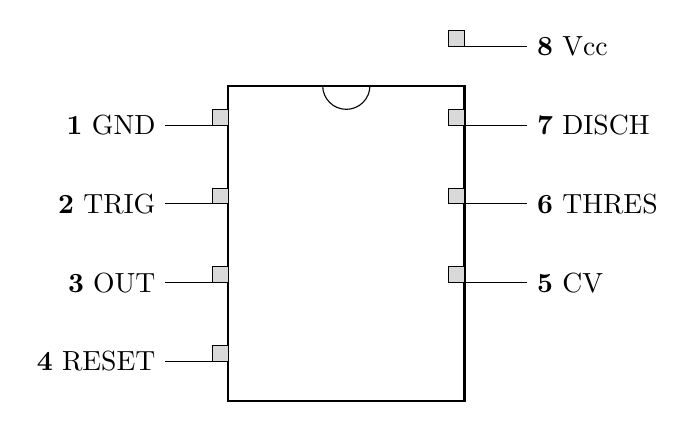
\begin{tikzpicture}
    % IC Body
    \draw[thick] (0,0) rectangle (3,4);
    \draw (1.2,4) arc (180:360:0.3); % Notch
    
    % Left Pins
    \foreach \i/\label in {1/GND, 2/TRIG, 3/OUT, 4/RESET} {
        \draw (0, 4.5-\i) -- (-0.8, 4.5-\i);
        \node[left] at (-0.8, 4.5-\i) {\textbf{\i} \label};
        \filldraw (0, 4.5-\i) ++(-0.2,0) rectangle ++(0.2,0.2) [fill=gray!30];
    }
    
    % Right Pins
    \foreach \i/\label in {8/Vcc, 7/DISCH, 6/THRES, 5/CV} {
        \draw (3, \i-4.5+1) -- (3.8, \i-4.5+1);
        \node[right] at (3.8, \i-4.5+1) {\textbf{\i} \label};
        \filldraw (3, \i-4.5+1) ++(0,0) rectangle ++(-0.2,0.2) [fill=gray!30];
    }
\end{tikzpicture}
\captionof{figure}{Pin Configuration of 555 Timer}
\end{center}

\textbf{Pin Explanations:}
\begin{enumerate}
    \item \textbf{GND (Ground):} Connected to the negative supply rail (0V).
    \item \textbf{Trigger:} A negative pulse (voltage < 1/3 Vcc) on this pin sets the internal Flip-Flop, making Output HIGH.
    \item \textbf{Output:} The output pin can source or sink current (up to 200mA) to drive loads.
    \item \textbf{Reset:} Active low pin. Connecting it to GND resets the timer (Output LOW). Normally connected to Vcc.
    \item \textbf{Control Voltage (CV):} Allows access to the 2/3 Vcc internal divider point. Usually connected to GND via a 0.01$\mu$F capacitor for noise immunity.
    \item \textbf{Threshold:} Checks voltage across the external capacitor. If voltage > 2/3 Vcc, it resets the internal Flip-Flop (Output LOW).
    \item \textbf{Discharge:} Connected to the open collector of the internal NPN transistor. Discharges the external capacitor when Output is LOW.
    \item \textbf{Vcc:} Power supply pin (+5V to +15V).
\end{enumerate}

\begin{mnemonicbox}
\mnemonic{Pins: G-T-O-R | C-T-D-V (Ground, Trigger, Out, Reset | Ctrl, Thres, Disch, Vcc)}
\end{mnemonicbox}
\end{solutionbox}

\questionmarks{1(c)}{7}{Draw and Explain block diagram of IC 555 timer.}

\begin{solutionbox}
The internal block diagram consists of resistors, comparators, an SR flip-flop, and an output stage.

\textbf{Block Diagram:}

\begin{center}
\begin{tikzpicture}[auto, node distance=1.5cm]
    % Components
    \node [gtu block] (div) {Voltage Divider\\(3 $\times$ 5k$\Omega$)};
    \node [gtu block, right=1cm of div] (comp1) {Comparator 1\\(Threshold)};
    \node [gtu block, below=1cm of comp1] (comp2) {Comparator 2\\(Trigger)};
    \node [gtu block, right=1.5cm of comp1] (ff) {SR Flip-Flop};
    \node [gtu block, right=1.5cm of ff] (out) {Output Stage\\(Inverter)};
    \node [gtu block, below=1cm of out] (disch) {Discharge\\Transistor};

    % Wiring (Simplified for conceptual view)
    % Vcc line
    \node[above=0.5cm of div] (vcc) {Vcc (8)};
    \draw [gtu arrow] (vcc) -- (div);
    
    % Divider taps
    \draw [->] (div.east) -- (comp1.west) node[midway, above, font=\tiny] {2/3 Vcc};
    \draw [->] (div.south east) -- (comp2.west) node[midway, below, font=\tiny] {1/3 Vcc};
    
    % Inputs
    \node[above=0.5cm of comp1] (thres) {Threshold (6)};
    \draw [gtu arrow] (thres) -- (comp1);
    
    \node[below=0.5cm of comp2] (trig) {Trigger (2)};
    \draw [gtu arrow] (trig) -- (comp2);
    
    % Flip Flop Connections
    \draw [gtu arrow] (comp1) -- (ff) node[midway, above, font=\tiny] {R};
    \draw [gtu arrow] (comp2) -- (ff) node[midway, below, font=\tiny] {S};
    
    \node[above=0.5cm of ff] (rst) {Reset (4)};
    \draw [gtu arrow] (rst) -- (ff);
    
    % Output
    \draw [gtu arrow] (ff) -- (out);
    \node[right=0.5cm of out] (outpin) {Output (3)};
    \draw [gtu arrow] (out) -- (outpin);
    
    % Discharge
    \draw [->] (ff.south) |- (disch.west);
    \node[right=0.5cm of disch] (dischpin) {Discharge (7)};
    \draw [gtu arrow] (disch) -- (dischpin);
    
\end{tikzpicture}
\captionof{figure}{Functional Block Diagram of 555 Timer}
\end{center}

\textbf{Explanation of Blocks:}
\begin{enumerate}
    \item \textbf{Voltage Divider:} Three 5k$\Omega$ resistors divide Vcc into 2/3 Vcc and 1/3 Vcc references.
    \item \textbf{Comparators:} 
        \begin{itemize}
            \item \textbf{Upper Comparator (Threshold):} Compares input at Pin 6 with 2/3 Vcc. If Pin 6 > 2/3 Vcc, Output resets (LOW).
            \item \textbf{Lower Comparator (Trigger):} Compares input at Pin 2 with 1/3 Vcc. If Pin 2 < 1/3 Vcc, Output sets (HIGH).
        \end{itemize}
    \item \textbf{SR Flip-Flop:} Stores the state determined by the comparators. Reset pin (4) can force it to reset state.
    \item \textbf{Output Stage:} A power amplifier/inverter buffer to drive external loads (Pin 3).
    \item \textbf{Discharge Transistor:} An NPN transistor that switches ON when output is LOW, providing a discharge path for the external capacitor (Pin 7).
\end{enumerate}
\end{solutionbox}

\questionmarks{1(c OR)}{7}{Draw and Explain A-stable and mono-stable multivibrator using 555 timer IC.}

\begin{solutionbox}
\textbf{1. Astable Multivibrator (Free Running Oscillator)}
\begin{itemize}
    \item No stable state; oscillates between HIGH and LOW.
    \item \textbf{Circuit:} Pins 2 and 6 are tied together to a capacitor $C$. Two resistors $R_1$ and $R_2$ charge $C$, and $R_2$ discharges it.
\end{itemize}

\begin{center}
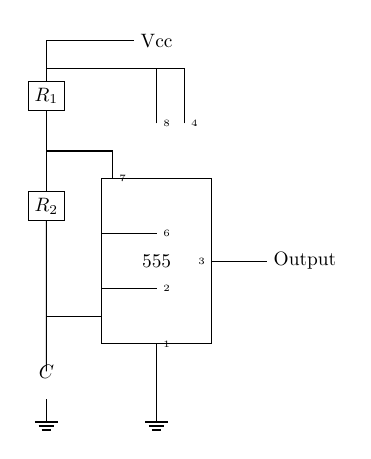
\begin{tikzpicture}[scale=0.7, transform shape]
    \node[draw, minimum width=2cm, minimum height=3cm] (ic) at (0,0) {555};
    
    % Components for Astable
    \node (vcc) at (0, 4) {Vcc};
    \node[draw, rectangle] (r1) at (-2, 3) {$R_1$};
    \node[draw, rectangle] (r2) at (-2, 1) {$R_2$};
    \node (cap) at (-2, -2) {$C$};
    \draw (-2,-2.5) node[ground]{};
    
    % Connections
    \draw (vcc) -| (r1);
    \draw (r1) -- (r2);
    \draw (r2) -- (-2, -1.8) -- (-2, -2);
    
    % Pin 7 to between R1 and R2
    \draw (0, 1.5) -- (-0.8, 1.5) node[right, font=\tiny] {7} -- (-0.8, 2) -| (-2, 2);
    
    % Pin 6 and 2 to between R2 and C
    \draw (0, 0.5) node[right, font=\tiny] {6} -- (-1, 0.5) -- (-1, -1) -- (-2, -1);
    \draw (0, -0.5) node[right, font=\tiny] {2} -- (-1, -0.5) -- (-1, -1);
    
    % Pin 8 and 4 to Vcc
    \draw (0, 2.5) node[right, font=\tiny] {8} -- (0, 3.5) -- (-2, 3.5);
    \draw (0.5, 2.5) node[right, font=\tiny] {4} -- (0.5, 3.5) -| (0, 3.5);

    % Pin 1 to GND
    \draw (0, -1.5) node[right, font=\tiny] {1} -- (0, -2.5) node[ground]{};
    
    % Pin 3 Out
    \draw (1, 0) node[left, font=\tiny] {3} -- (2, 0) node[right] {Output};
\end{tikzpicture}
\captionof{figure}{Astable Multivibrator}
\end{center}

\textbf{Operation:} Capacitor charges via $R_1+R_2$ (Output HIGH) and discharges via $R_2$ (Output LOW).
Duty cycle depends on ratio of $R_1$ and $R_2$.

\textbf{2. Monostable Multivibrator (One-Shot)}
\begin{itemize}
    \item One stable state (LOW). Trigger (Pin 2) creates a temporary HIGH pulse.
    \item \textbf{Circuit:} Trigger applied to Pin 2. Resistor $R$ and Capacitor $C$ determine pulse width $T = 1.1 RC$.
\end{itemize}

\begin{center}
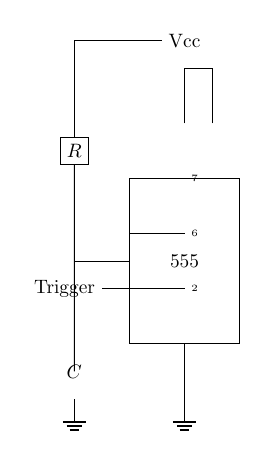
\begin{tikzpicture}[scale=0.7, transform shape]
    \node[draw, minimum width=2cm, minimum height=3cm] (ic) at (0,0) {555};
    
    % Components
    \node (vcc) at (0, 4) {Vcc};
    \node[draw, rectangle] (r) at (-2, 2) {$R$};
    \node (cap) at (-2, -2) {$C$};
    \draw (-2,-2.5) node[ground]{};
    
    % Connections
    \draw (vcc) -| (r);
    \draw (r) -- (-2, -1.8) -- (-2, -2);
    
    % Pin 6 and 7 to between R and C
    \draw (0, 1.5) node[right, font=\tiny] {7} -- (-1, 1.5) -- (-1, 0) -- (-2, 0);
    \draw (0, 0.5) node[right, font=\tiny] {6} -- (-1, 0.5) -- (-1, 0);
    
    % Pin 2 Trigger
    \draw (0, -0.5) node[right, font=\tiny] {2} -- (-1, -0.5) -- (-1.5, -0.5) node[left] {Trigger};
    
    % Pin 8 and 4
    \draw (0, 2.5) -- (0, 3.5);
    \draw (0.5, 2.5) -- (0.5, 3.5) -| (0, 3.5);
    
    % Pin 1
    \draw (0, -1.5) -- (0, -2.5) node[ground]{};
\end{tikzpicture}
\captionof{figure}{Monostable Multivibrator}
\end{center}

\textbf{Operation:} Output is normally LOW. A negative trigger sets Output HIGH. Capacitor charges through $R$. When $V_C = 2/3 Vcc$, Output resets to LOW and C discharges.
\end{solutionbox}

% ==================================================================
% Q.2
% ==================================================================

\questionmarks{2(a)}{3}{Write short note on Active components and passive components.}

\begin{solutionbox}
Electronic components are classified into two types based on their energy handling capability:

\textbf{1. Active Components:}
\begin{itemize}
    \item Components that can \textbf{control} the flow of current or \textbf{amplify} a signal.
    \item They require an external power source to operate.
    \item \textbf{Examples:} Transistors (BJT, FET), Diodes (Zener, LED), ICs (Integrated Circuits), Op-Amps.
\end{itemize}

\textbf{2. Passive Components:}
\begin{itemize}
    \item Components that can only \textbf{store} or \textbf{dissipate} energy. They cannot control current or amplify signals.
    \item They do not require an external power source to function.
    \item \textbf{Examples:} Resistors (Dissipate energy), Capacitors (Store electric energy), Inductors (Store magnetic energy).
\end{itemize}

\begin{center}
\captionof{table}{Comparison of Active and Passive Components}
\begin{tabulary}{\linewidth}{|L|L|L|}
\hline
\textbf{Parameter} & \textbf{Active Components} & \textbf{Passive Components} \\ \hline
Function & Amplify/Switch signals & Store/Dissipate energy \\ \hline
Gain & Can provide power gain & No power gain (Gain < 1) \\ \hline
Control & Control currrent flow & Cannot control current \\ \hline
Example & Transistor, Diode & Resistor, Capacitor \\ \hline
\end{tabulary}
\end{center}
\end{solutionbox}

\questionmarks{2(b)}{4}{Write color band of following resistance. (1) 47 $\Omega \pm 5\%$}

\begin{solutionbox}
To find the color code for $47 \Omega \pm 5\%$:

\begin{itemize}
    \item \textbf{Value:} 47 $\Omega$
    \item \textbf{Digit 1:} 4 corresponds to \textbf{Yellow}.
    \item \textbf{Digit 2:} 7 corresponds to \textbf{Violet}.
    \item \textbf{Multiplier:} To get 47, we need $47 \times 10^0 = 47$. So multiplier is $10^0$, which corresponds to \textbf{Black}.
        \begin{itemize}
            \item Alternatively, if interpreted as Band 3 being multiplier for ohms: $47 \times 1 = 47$. (Yellow, Violet, Black).
            \item Note: Sometimes $47\Omega$ might be represented as Yellow, Violet, Gold ($47 \times 0.1 = 4.7$ - Incorrect). Correct is $47 \times 1$.
        \end{itemize}
    \item \textbf{Tolerance:} $\pm 5\%$ corresponds to \textbf{Gold}.
\end{itemize}

\textbf{Answer:}
\begin{center}
    \textbf{Yellow - Violet - Black - Gold}
\end{center}

\begin{mnemonicbox}
\mnemonic{BBROYGBVGW: Black Brown Red Orange Yellow Green Blue Violet Grey White}
\end{mnemonicbox}
\end{solutionbox}

\questionmarks{2(c)}{7}{Explain working of Full wave center tap rectifier with circuit diagram and wave form.}

\begin{solutionbox}
A Full Wave Center Tap Rectifier uses two diodes and a center-tapped transformer to convert the entire AC cycle into pulsating DC.

\textbf{Circuit Diagram:}
\begin{center}
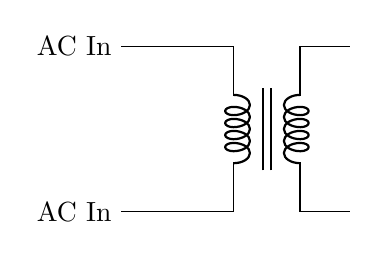
\begin{tikzpicture}[scale=0.8]
    % Transformer
    \draw (0,0) node[transformer core](T){};
    
    % Primary
    \draw (T.A1) -- ++(-1,0) node[left] {AC In};
    \draw (T.A2) -- ++(-1,0) node[left] {AC In};
    
    % Secondary
    \coordinate (S1) at (T.B1);
    \coordinate (S2) at (T.B2);
    \coordinate (CT) at ($(S1)!0.5!(S2)$); % Center tap approximation visual is tricky with tikz components, doing manual
\end{tikzpicture}
% Redrawing simple transformer manually for better control
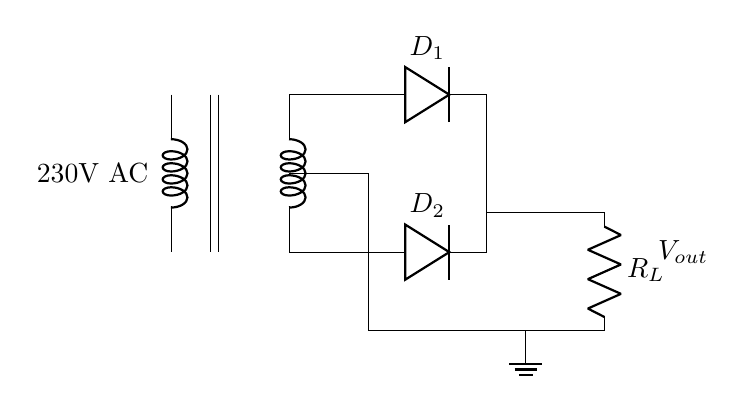
\begin{tikzpicture}
    % Transformer Coils
    \draw (0,2) to[L] (0,0); % Primary
    \draw (0.5,2) -- (0.5,0); \draw (0.6,2) -- (0.6,0); % Core
    \draw (1.5,2) to[L, name=L2] (1.5,0); % Secondary
    
    % Center Tap
    \coordinate (CT) at (1.5,1); % Midpoint of secondary visually
    \draw (CT) -- (2.5,1) -- (2.5,-1) -- (5.5,-1); % GND path
    \node at (4.5,-1) [ground]{};
    
    % Diodes
    \draw (1.5,2) -- (2.5,2) to[D, l=$D_1$] (4,2) -- (4,0.5);
    \draw (1.5,0) -- (2.5,0) to[D, l=$D_2$] (4,0) -- (4,0.5);
    
    % Load
    \draw (4,0.5) -- (5.5,0.5) to[R, l=$R_L$] (5.5,-1);
    
    % Labels
    \node at (-1,1) {230V AC};
    \node at (6.5,0) {$V_{out}$};
\end{tikzpicture}
\captionof{figure}{Full Wave Center Tap Rectifier}
\end{center}

\textbf{Operation:}
\begin{itemize}
    \item \textbf{Positive Half Cycle:} Point A (Top) is positive w.r.t CT. $D_1$ is Forward Biased (ON), $D_2$ is Reverse Biased (OFF). Current flows through $D_1$ and $R_L$.
    \item \textbf{Negative Half Cycle:} Point B (Bottom) is positive w.r.t CT. $D_2$ is Forward Biased (ON), $D_1$ is Reverse Biased (OFF). Current flows through $D_2$ and $R_L$.
    \item Current flows through $R_L$ in the \textbf{same direction} during both half cycles.
\end{itemize}

\textbf{Waveforms:}
\begin{center}
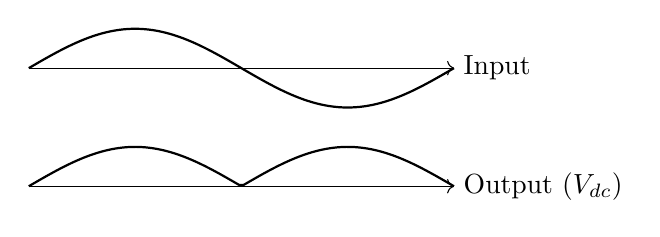
\begin{tikzpicture}[xscale=0.015, yscale=0.5]
    % Input
    \draw[->] (0,3) -- (360,3) node[right] {Input};
    \draw[thick] plot[domain=0:360, samples=100] (\x, {3 + sin(\x)});
    
    % Output
    \draw[->] (0,0) -- (360,0) node[right] {Output ($V_{dc}$)};
    \draw[thick] plot[domain=0:360, samples=100] (\x, {abs(sin(\x))});
\end{tikzpicture}
\captionof{figure}{Input and Output Waveforms}
\end{center}
\end{solutionbox}

\questionmarks{2(a OR)}{3}{Explain concept of capacitors.}

\begin{solutionbox}
A capacitor is a passive component that stores electrical energy in an electric field.

\begin{itemize}
    \item \textbf{Structure:} Consists of two conductive plates separated by an insulating material called a \textbf{dielectric} (Air, Paper, Mica, Ceramic).
    \item \textbf{Function:} It opposes any change in voltage. It blocks DC and passes AC.
    \item \textbf{Capacitance ($C$):} The ability to store charge. $C = Q/V$. Unit is Farad (F).
    \item \textbf{Charging/Discharging:} When voltage is applied, it charges up to the source voltage. When the path is closed, it discharges.
\end{itemize}
\end{solutionbox}

\questionmarks{2(b OR)}{4}{Calculate value of resistor and tolerance for following color bands on resistor: (1) Brown, Green, yellow, gold (2) Grey, blue, brown}

\begin{solutionbox}
\textbf{1. Brown, Green, Yellow, Gold}
\begin{itemize}
    \item \textbf{Brown (1st Band):} 1
    \item \textbf{Green (2nd Band):} 5
    \item \textbf{Yellow (Multiplier):} $\times 10^4$ (10,000)
    \item \textbf{Gold (Tolerance):} $\pm 5\%$
    \item \textbf{Calculation:} $15 \times 10,000 = 150,000 \Omega$
    \item \textbf{Answer:} \textbf{150 k$\Omega$ $\pm 5\%$}
\end{itemize}

\textbf{2. Grey, Blue, Brown}
\begin{itemize}
    \item \textbf{Grey (1st Band):} 8
    \item \textbf{Blue (2nd Band):} 6
    \item \textbf{Brown (Multiplier):} $\times 10^1$ (10)
    \item \textbf{Tolerance:} No 4th band implies $\pm 20\%$ (Standard convention for 3-band).
    \item \textbf{Calculation:} $86 \times 10 = 860 \Omega$
    \item \textbf{Answer:} \textbf{860 $\Omega$ $\pm 20\%$}
\end{itemize}
\end{solutionbox}

\questionmarks{2(c OR)}{7}{Explain working of Full wave bridge rectifier with circuit diagram and wave form.}

\begin{solutionbox}
A Full Wave Bridge Rectifier uses four diodes ($D_1, D_2, D_3, D_4$) in a bridge configuration. It does not require a center-tapped transformer.

\textbf{Circuit Diagram:}
\begin{center}
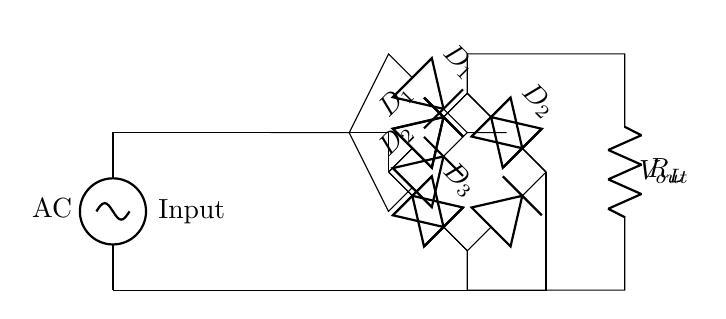
\begin{tikzpicture}
    % AC Source
    \draw (-2,0) to[sV, l=AC] (-2,2) -- (0,2);
    \draw (-2,0) -- (0,0);
    
    % Bridge
    \draw (0,2) -- (1,2) -- (1.5,3) to[D, l=$D_1$] (2.5,2) -- (3,2); % Top Left
    \draw (1,2) -- (1.5,1) to[D, l=$D_2$] (2.5,2); % Bottom Left diode D2 actually points differently dependent on config
    % Standard Bridge:
    % Left node: Input 1. Right node: Input 2? No.
    % Top node: + DC. Bottom node: - DC.
    % Let's draw standard diamond.
    \draw (1.5,1.5) to[D, l=$D_1$] (2.5, 2.5); % Left to Top
    \draw (2.5,2.5) to[D, l=$D_2$] (3.5, 1.5); % Top to Right
    \draw (1.5,1.5) to[D, l=$D_3$] (2.5, 0.5); % Left to Bottom (Reverse) -> Wait.
    % Let's trace paths.
    % Left Input (1.5, 1.5). Right Input (3.5, 1.5).
    % Top Output (2.5, 2.5). Bottom Output (2.5, 0.5).
    
    % D1: Left -> Top. Anode at Left? NO. Diodes point to Positive.
    % So Left -> Top (Anode to Cathode).
    \draw (1.5,1.5) to[D] (2.5, 2.5); 
    % Right -> Top.
    \draw (3.5,1.5) to[D] (2.5, 2.5);
    
    % Bottom -> Left.
    \draw (2.5,0.5) to[D] (1.5, 1.5);
    % Bottom -> Right.
    \draw (2.5,0.5) to[D] (3.5, 1.5);
    
    % Inputs
    \draw (0,2) -| (1.5,1.5); % Top AC wire to Left Bridge Node
    \draw (0,0) -| (3.5,1.5); % Bottom AC wire to Right Bridge Node -- careful crossing lines
    
    % Load
    \draw (2.5, 2.5) -- (2.5, 3) -- (4.5, 3) to[R, l=$R_L$] (4.5, 0) -- (2.5, 0) -- (2.5, 0.5);
    
    % Labels
    \node at (-1,1) {Input};
    \node at (5, 1.5) {$V_{out}$};
\end{tikzpicture}
\captionof{figure}{Bridge Rectifier Circuit}
\end{center}

\textbf{Operation:}
\begin{itemize}
    \item \textbf{Positive Half Cycle:} Current flows via $D_1 \rightarrow R_L \rightarrow D_3$ (assuming standard label). Two diodes conduct. Path is closed.
    \item \textbf{Negative Half Cycle:} Current flows via $D_2 \rightarrow R_L \rightarrow D_4$ (assuming standard label). Other two diodes conduct.
    \item Result is pulsating DC at the output.
\end{itemize}

\textbf{Advantages:}
\begin{itemize}
    \item No center-tap transformer needed.
    \item Higher PIV (Peak Inverse Voltage) rating efficiency compared to center-tap ($PIV = V_m$ vs $2V_m$).
\end{itemize}
\end{solutionbox}

% ==================================================================
% Q.3
% ==================================================================

\questionmarks{3(a)}{3}{Explain Light dependent resistor (LDR).}

\begin{solutionbox}
LDR (Light Dependent Resistor) is a passive component whose resistance changes with the intensity of light falling on it.

\begin{itemize}
    \item \textbf{Principle:} Photoconductivity. When light falls on the material (Cadmium Sulfide - CdS), electron-hole pairs are generated, increasing conductivity (decreasing resistance).
    \item \textbf{Dark Resistance:} Very high (M$\Omega$ range) in darkness.
    \item \textbf{Light Resistance:} Low (k$\Omega$ or $\Omega$ range) in bright light.
    \item \textbf{Symbol:}
    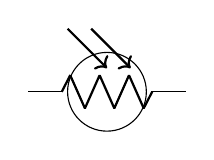
\begin{tikzpicture}[baseline]
        \draw (0,0) to[R] (2,0);
        \draw[->, thick] (0.5, 0.8) -- (1, 0.3);
        \draw[->, thick] (0.8, 0.8) -- (1.3, 0.3);
        \draw (1,0) circle (0.5);
    \end{tikzpicture}
    \item \textbf{Uses:} Street light control, burglar alarms, camera exposure control.
\end{itemize}
\end{solutionbox}

\questionmarks{3(b)}{4}{Explain half wave rectifier circuit with wave form.}

\begin{solutionbox}
A Half Wave Rectifier converts only one half of the AC cycle into DC.

\textbf{Circuit Diagram:}
\begin{center}
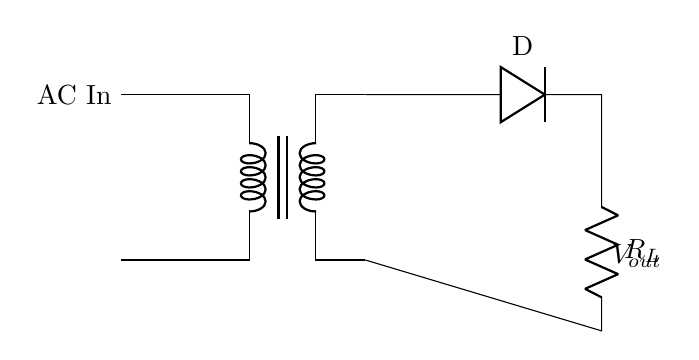
\begin{tikzpicture}
    % Transformer
    \draw (0,0) node[transformer core](T){};
    \draw (T.A1) -- ++(-1,0) node[left] {AC In}; \draw (T.A2) -- ++(-1,0);
    
    % Circuit
    \draw (T.B1) -- ++(1,0) to[D, l=D] ++(2,0) -- ++(0, -1) to[R, l=$R_L$] ++(0, -2) -- (T.B2);
    \node at (4.5, -1) {$V_{out}$};
\end{tikzpicture} 
\captionof{figure}{Half Wave Rectifier}
\end{center}

\textbf{Operation:}
\begin{itemize}
    \item During Positive half cycle: Diode is Forward Biased (ON). Current flows through $R_L$.
    \item During Negative half cycle: Diode is Reverse Biased (OFF). No current flows.
\end{itemize}

\textbf{Waveform:} output voltage appears only for 0 to $\pi$, zero for $\pi$ to $2\pi$.
\end{solutionbox}

\questionmarks{3(c)}{7}{List different types of clipper circuits and draw any two types of clipper circuits with its wave forms.}

\begin{solutionbox}
\textbf{Types of Clipper Circuits:}
\begin{enumerate}
    \item Series Clipper (Positive/Negative)
    \item Shunt (Parallel) Clipper (Positive/Negative)
    \item Biased Clipper (Positive/Negative)
    \item Combination (Dual) Clipper
\end{enumerate}

\textbf{1. Positive Shunt Clipper:}
\begin{itemize}
    \item Removes the positive half cycle.
\end{itemize}
\begin{center}
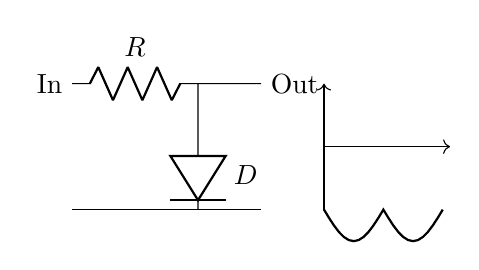
\begin{tikzpicture}[scale=0.8]
    % Circuit
    \draw (0,2) to[R, l=$R$] (2,2) -- (3,2);
    \draw (2,2) -- (2,1) to[D, l=$D$] (2,0);
    \draw (0,0) -- (3,0);
    \draw (0,2) node[left] {In}; \draw (3,2) node[right] {Out};
    
    % Waveform
    \begin{scope}[xshift=4cm]
        \draw[->] (0,1) -- (2,1); \draw[->] (0,0) -- (0,2);
        \draw[thick] plot[domain=0:2*pi, xscale=0.3, yscale=0.5] (\x, {-abs(sin(\x r))}); % Negative only? No, D conducts for Positive, shorting it. So output is 0 for positive. Neg cycle D is off, Output = Input.
        % Correct plot: 0 for 0-pi, -sin for pi-2pi
    \end{scope}
\end{tikzpicture}
\end{center}
For Positive Input: D is ON (Short), $V_{out} = 0$. For Negative Input: D is OFF (Open), $V_{out} = V_{in}$.

\textbf{2. Positive Series Clipper:}
\begin{itemize}
    \item Diode in series, reverse direction.
\end{itemize}
\begin{center}
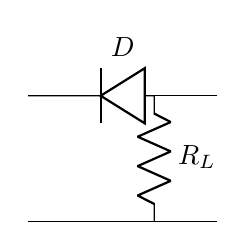
\begin{tikzpicture}[scale=0.8]
    % Circuit
    \draw (0,0) -- (3,0);
    \draw (0,2) -- (1,2) to[D, l=$D$, invert] (2,2) to[R, l=$R_L$] (2,0);
    \draw (2,2) -- (3,2);
    
    % Operation
    % For Positive: D (Cathode to input) is Reverse Biased (OFF). Vout = 0.
    % For Negative: D is Forward Biased (ON). Vout = Vin.
\end{tikzpicture}
\captionof{figure}{Positive Series Clipper}
\end{center}
\end{solutionbox}

\questionmarks{3(a OR)}{3}{Explain self and mutual inductance in brief.}

\begin{solutionbox}
\textbf{Self Inductance ($L$):} The property of a coil to oppose any change in current flowing through \textbf{itself} by inducing an EMF. $e = -L \frac{di}{dt}$.

\textbf{Mutual Inductance ($M$):} The property of a coil to oppose current change in a \textbf{neighboring} coil by inducing an EMF in itself due to magnetic coupling. $e_2 = -M \frac{di_1}{dt}$.
\end{solutionbox}

\questionmarks{3(b OR)}{4}{Explain the following terms in brief. (1) Ripple factor (2) Ripple frequency}

\begin{solutionbox}
\textbf{1. Ripple Factor ($\gamma$):}
\begin{itemize}
    \item It is the ratio of the RMS value of the AC component of the output to the DC component of the output.
    \item $\gamma = \frac{V_{ac(rms)}}{V_{dc}}$. It indicates the purity of the DC output (Lower is better).
\end{itemize}

\textbf{2. Ripple Frequency ($f_r$):}
\begin{itemize}
    \item The frequency of the AC ripples present in the DC output.
    \item For Half Wave: $f_r = f_{in}$ (e.g., 50 Hz).
    \item For Full Wave: $f_r = 2f_{in}$ (e.g., 100 Hz).
\end{itemize}
\end{solutionbox}

\questionmarks{3(c OR)}{7}{List different types of clamper circuits and draw any two types of clamper circuits with its wave forms.}

\begin{solutionbox}
Clampers shift the DC level of a signal without changing its shape.
\textbf{Types:} Positive Clamper, Negative Clamper, Biased Clamper.

\textbf{1. Positive Clamper:}
\begin{itemize}
    \item Shifts the waveform up.
\end{itemize}
\begin{center}
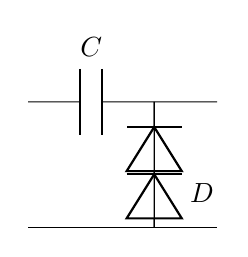
\begin{tikzpicture}[scale=0.8]
    % Circuit
    \draw (0,2) to[C, l=$C$] (2,2) -- (3,2);
    \draw (2,2) -- (2,1) to[D, l=$D$, invert] (2,0); % Diode pointing up for Pos Clamper?
    % Pos Clamper: Diode points "up" (Cathode at top? No. Anode at bottom?) 
    % During neg cycle, D conducts, charging C (Left -, Right +). Cap charges to Vm.
    % Then Vout = Vin + Vm.
    % Circuit: C in series. Diode in shunt.
    
    % Diode Anode to GND, Cathode to Signal -> D points up.
    % Wait. If D points up:
    % Neg cycle (Vin < 0): Anode(0) > Cathode(Neg). D ON. C charges to Vm (Right +).
    % Pos cycle (Vin > 0): D OFF. Vout = Vin + Vc = Vin + Vm. (Shift Up). Correct.
    \draw (2,0) -- (2,0.5) to[D] (2,2); % Points up means Anode bottom? No triangle points direction of current.
    % Correct: Anode (Triangle base) at Bottom (GND). Cathode (Bar) at Top.
    % Is this "pointing up"? Triangle points up. Current flows up? No, current conventional flows Anode->Cathode.
    % So Triangle base at bottom, Tip at top.
    
    \draw (0,0) -- (3,0);
\end{tikzpicture}
\captionof{figure}{Positive Clamper}
\end{center}

\textbf{2. Negative Clamper:}
\begin{itemize}
    \item Shifts the waveform down.
    \item Diode direction reversed (Cathode at GND).
\end{itemize}
\end{solutionbox}

% ==================================================================
% Q.4
% ==================================================================

\questionmarks{4(a)}{3}{Draw Symbols of Zener diode, LED, and Varactor diode.}

\begin{solutionbox}
\begin{center}
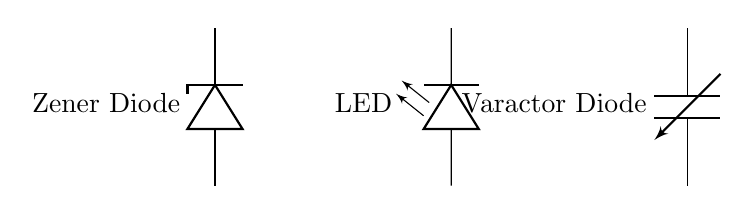
\begin{tikzpicture}
    % Zener
    \draw (0,0) to[zD, l=Zener Diode] (0,2);
    
    % LED
    \draw (3,0) to[leD, l=LED] (3,2);
    
    % Varactor
    \draw (6,0) to[vC, l=Varactor Diode, invert] (6,2); % vC is varactor
    % Note: Variable Capacitor symbol or diode with capacitor bar
\end{tikzpicture}
\end{center}
\end{solutionbox}

\questionmarks{4(b)}{4}{Explain Photodiode.}

\begin{solutionbox}
A Photodiode is a PN junction diode that converts light energy into electrical current.
\begin{itemize}
    \item \textbf{Operation:} It is operated in \textbf{Reverse Bias}.
    \item \textbf{Working:} When light falls on the junction, energy breaks covalent bonds, creating electron-hole pairs. These carriers are swept by the electric field, creating a reverse current proportional to light intensity.
    \item \textbf{Dark Current:} Small leakage current that flows even when no light is present.
    \item \textbf{Applications:} Optical communication, remote controls, smoke detectors.
\end{itemize}
\end{solutionbox}

\questionmarks{4(c)}{7}{Explain construction, characteristics and working of Zener diode.}

\begin{solutionbox}
\textbf{Zener Diode:} A heavily doped PN junction diode designed to operate in the reverse breakdown region.

\textbf{Construction:}
\begin{itemize}
    \item Heavily doped P and N regions to create a narrow depletion region.
    \item Encapsulated in glass or plastic.
\end{itemize}

\textbf{Working:}
\begin{itemize}
    \item \textbf{Forward Bias:} Acts like a normal diode.
    \item \textbf{Reverse Bias:}
    \item At low voltage, negligible current flows.
    \item At Breakdown Voltage ($V_z$), current increases sharply (Avalanche/Zener breakdown). The voltage across it remains constant ($V_z$) despite large changes in current.
\end{itemize}

\textbf{V-I Characteristics:}
\begin{center}
\begin{tikzpicture}[scale=0.7]
    \draw[->] (-4,0) -- (2,0) node[right] {$V$};
    \draw[->] (0,-3) -- (0,3) node[above] {$I$};
    
    % Forward
    \draw[thick] (0,0) -- (0.5,0) to[out=0,in=270] (1,2);
    \node at (1.2,1) {Forward};
    
    % Reverse
    \draw[thick] (0,0) -- (-2,0) -- (-2,-2.5);
    \node at (-2,-2.8) {$V_z$};
    \node[left] at (-2, -1) {Breakdown};
    
    \node at (2.5,-3) {Reverse};
\end{tikzpicture}
\captionof{figure}{V-I Characteristics of Zener Diode}
\end{center}
\end{solutionbox}

\questionmarks{4(a OR)}{3}{List applications of LED and Varactor diode.}

\begin{solutionbox}
\textbf{LED (Light Emitting Diode):}
\begin{itemize}
    \item Indicators and Displays (7-segment).
    \item Lighting (Bulbs, Torch).
    \item Optical Communication (Fiber optics).
    \item Remote Controls (IR LED).
\end{itemize}

\textbf{Varactor Diode (Varicap):}
\begin{itemize}
    \item Tuning circuits (FM/TV receivers).
    \item Voltage Controlled Oscillators (VCO).
    \item Frequency Multipliers.
    \item Adjustable Bandpass Filters.
\end{itemize}
\end{solutionbox}

\questionmarks{4(b OR)}{4}{Explain Zener diode as a voltage regulator.}

\begin{solutionbox}
Zener diode maintains a constant output voltage ($V_z$) irrespective of changes in input voltage ($V_{in}$) or load current ($I_L$).

\textbf{Circuit:}
\begin{center}
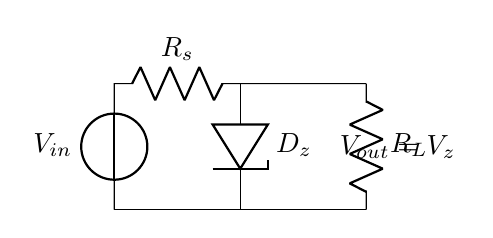
\begin{tikzpicture}[scale=0.8]
    \draw (-2,0) to[V, l=$V_{in}$] (-2,2) to[R, l=$R_s$] (0,2) -- (2,2);
    \draw (0,2) to[zD, l=$D_z$] (0,0); % Zener in parallel
    \draw (2,2) to[R, l=$R_L$] (2,0);
    \draw (-2,0) -- (2,0);
    \node at (2.5,1) {$V_{out} = V_z$};
\end{tikzpicture}
\end{center}

\textbf{Working:}
\begin{itemize}
    \item If $V_{in}$ increases, Current rises. Zener absorbs extra current. Voltage drop across Series Resistor ($R_s$) increases. $V_{out}$ remains $V_z$.
    \item If Load current ($I_L$) changes, Zener current ($I_z$) adjusts such that $I_s = I_z + I_L$ keeps voltage constant.
\end{itemize}
\end{solutionbox}

\questionmarks{4(c OR)}{7}{Explain construction, characteristics and working of Varactor diode.}

\begin{solutionbox}
\textbf{Varactor Diode:} A variable capacitance diode. It acts as a voltage-dependent capacitor.

\textbf{Working Principle:}
\begin{itemize}
    \item Operates in \textbf{Reverse Bias}.
    \item The depletion region acts as a dielectric. P and N regions act as plates.
    \item \textbf{Capacitance Formula:} $C_T = \frac{\epsilon A}{W}$.
    \item Increasing Reverse Voltage ($V_R$) $\rightarrow$ Width of Depletion Region ($W$) Increases $\rightarrow$ Capacitance ($C_T$) Decreases.
    \item $C \propto \frac{1}{\sqrt{V_R}}$.
\end{itemize}

\textbf{Characteristics:}
\begin{center}
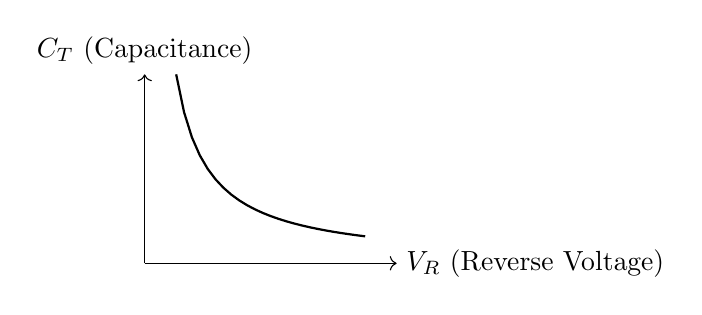
\begin{tikzpicture}[scale=0.8]
    \draw[->] (0,0) -- (4,0) node[right] {$V_R$ (Reverse Voltage)};
    \draw[->] (0,0) -- (0,3) node[above] {$C_T$ (Capacitance)};
    \draw[thick] plot[domain=0.5:3.5] (\x, {1.5/\x}); % Curve decreasing
\end{tikzpicture}
\captionof{figure}{C-V Characteristics of Varactor Diode}
\end{center}
\end{solutionbox}

% ==================================================================
% Q.5
% ==================================================================

\questionmarks{5(a)}{3}{Explain transistor as a switch.}

\begin{solutionbox}
A transistor operates as a switch by shifting between \textbf{Cut-off} and \textbf{Saturation} regions.
\begin{itemize}
    \item \textbf{OFF State (Open Switch):} Operates in Cut-off region. $I_B = 0 \Rightarrow I_C = 0$. $V_{CE} = V_{CC}$.
    \item \textbf{ON State (Closed Switch):} Operates in Saturation region. $I_B$ is high enough such that $I_C$ is maximum ($V_{CC}/R_C$). $V_{CE} \approx 0$ (Saturation voltage).
\end{itemize}
\end{solutionbox}

\questionmarks{5(b)}{4}{Draw Common Emitter (CE) configuration of NPN transistors and its input characteristics.}

\begin{solutionbox}
\textbf{CE Configuration:} Emitter is common to both input and output.
\begin{center}
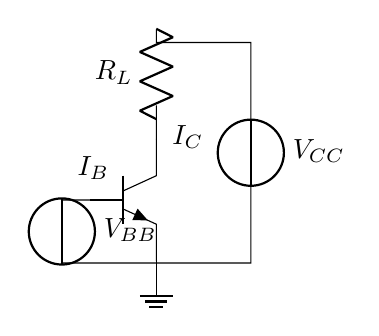
\begin{tikzpicture}[scale=0.8]
    \draw (0,0) node[npn](Q){};
    \draw (Q.E) -- (0,-1) node[ground]{}; % Emitter to GND
    \draw (Q.B) -- (-1.5,0) to[V, l=$V_{BB}$] (-1.5,-1) -- (0,-1); % Input loop
    \draw (Q.C) -- (0,1.5) to[R, l=$R_L$] (0,2.5) -- (1.5,2.5) to[V, l=$V_{CC}$] (1.5,-1) -- (0,-1); % Output loop
    
    \node at (-1, 0.5) {$I_B$};
    \node at (0.5, 1) {$I_C$};
    % Voltmeter VBE and VCE can be shown
\end{tikzpicture}
\end{center}

\textbf{Input Characteristics:} Graph of $I_B$ vs $V_{BE}$ at constant $V_{CE}$.
\begin{center}
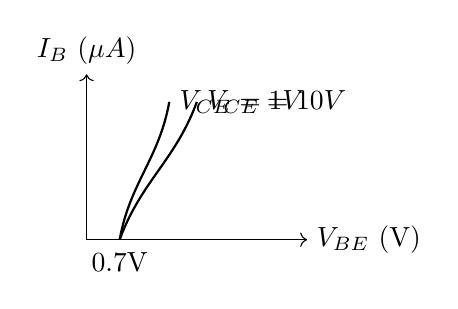
\begin{tikzpicture}[scale=0.7]
    \draw[->] (0,0) -- (4,0) node[right] {$V_{BE}$ (V)};
    \draw[->] (0,0) -- (0,3) node[above] {$I_B$ ($\mu A$)};
    
    \draw[thick] (0.6,0) to[out=80, in=260] (1.5, 2.5) node[right] {$V_{CE}=1V$};
    \draw[thick] (0.6,0) to[out=70, in=250] (2, 2.5) node[right] {$V_{CE}=10V$};
    
    \node at (0.6, -0.4) {0.7V}; % Knee voltage
\end{tikzpicture}
\end{center}
\end{solutionbox}

\questionmarks{5(c)}{7}{Draw symbol and construction of NPN Transistor and explain its working.}

\begin{solutionbox}
\textbf{Symbol:}
\begin{center}
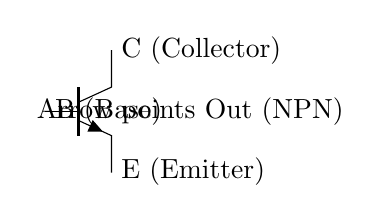
\begin{tikzpicture}
    \draw (0,0) node[npn](Q){};
    \node[right] at (Q.C) {C (Collector)};
    \node[right] at (Q.B) {B (Base)};
    \node[right] at (Q.E) {E (Emitter)};
    \node at (1, 0) {Arrow points Out (NPN)};
\end{tikzpicture}
\end{center}

\textbf{Construction:}
\begin{itemize}
    \item Consists of three layers: Two N-type regions separated by a P-type region.
    \item \textbf{Emitter:} Heavily doped (Supplies carriers).
    \item \textbf{Base:} Lightly doped and very thin (Controls carriers).
    \item \textbf{Collector:} Moderately doped and physically large (Collects carriers).
\end{itemize}

\textbf{Working (Active Mode):}
\begin{itemize}
    \item \textbf{Biasing:} Emitter-Base junction is Forward Biased ($V_{BE}$). Collector-Base junction is Reverse Biased ($V_{CB}$).
    \item Majority carriers (Electrons) from Emitter crossover to Base.
    \item Since Base is thin and lightly doped, only a few ($\approx 5\%$) recombine with Holes. $I_B$ is small.
    \item The rest ($\approx 95\%$) are attracted by the high positive potential of the Collector.
    \item $I_E = I_B + I_C$.
\end{itemize}
\end{solutionbox}

\questionmarks{5(a OR)}{3}{Compare CB, CE and CC configuration of transistor.}

\begin{solutionbox}
\begin{center}
\captionof{table}{Comparison of Transistor Configurations}
\begin{tabulary}{\linewidth}{|L|L|L|L|}
\hline
\textbf{Parameter} & \textbf{Common Base (CB)} & \textbf{Common Emitter (CE)} & \textbf{Common Collector (CC)} \\ \hline
Input Res. & Low & Medium & High \\ \hline
Output Res. & High & Medium & Low \\ \hline
Current Gain & Low ($\alpha < 1$) & High ($\beta$) & High ($\gamma$) \\ \hline
Voltage Gain & High & Medium & Low ($<1$) \\ \hline
Phase Shift & $0^\circ$ & $180^\circ$ & $0^\circ$ \\ \hline
Application & RF Amplifier & Audio Amplifier & Impedance Matching \\ \hline
\end{tabulary}
\end{center}
\end{solutionbox}

\questionmarks{5(b OR)}{4}{Explain transistor as a single stage common emitter amplifier.}

\begin{solutionbox}
\textbf{Circuit Diagram:}
\begin{center}
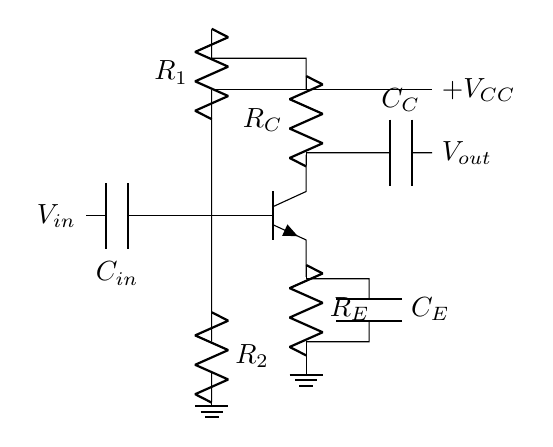
\begin{tikzpicture}[scale=0.8]
    % Simple CE Amp with biasing
    \draw (0,0) node[npn](Q){};
    \draw (Q.E) -- (0,-1) to[R, l=$R_E$] (0,-2) node[ground]{};
    \draw (0,-1) -- (1,-1) to[C, l=$C_E$] (1,-2) -- (0,-2); % Bypass Cap
    
    \draw (Q.C) -- (0,1) to[R, l=$R_C$] (0,2) -- (2,2) node[right] {$+V_{CC}$};
    \draw (0,1) -- (1,1) to[C, l=$C_C$] (2,1) node[right] {$V_{out}$};
    
    \draw (Q.B) -- (-1.5,0);
    \draw (-1.5,0) -- (-1.5, 2) to[R, l=$R_1$] (-1.5,2.5) -- (0,2.5) -- (0,2); % R1 to Vcc. Wait, simplified biasing used
    \draw (-1.5,0) -- (-1.5, -2) to[R, l=$R_2$] (-1.5,-2.5) node[ground]{}; % R2 to GND
    
    \draw (-1.5,0) -- (-2.5,0) to[C, l=$C_{in}$] (-3.5,0) node[left] {$V_{in}$};
    
    % Vcc line
    \draw (0,2) -- (-1.5, 2); 
\end{tikzpicture} 
\captionof{figure}{Single Stage CE Amplifier (Voltage Divider Bias)}
\end{center}

\textbf{Operation:}
\begin{itemize}
    \item $R_1, R_2$ form a voltage divider to bias the base.
    \item Input signal superimposes on the DC bias.
    \item During positive half of inputs, $V_{BE}$ increases $\rightarrow$ $I_B$ increases $\rightarrow$ $I_C$ increases $\rightarrow$ Voltage drop across $R_C$ increases $\rightarrow$ $V_{CE}$ decreases.
    \item Result: Output is $180^\circ$ phase shifted (Inverted) and amplified.
\end{itemize}
\end{solutionbox}

\questionmarks{5(c OR)}{7}{Explain common base (CB) configuration of NPN transistors with its input-output characteristics.}

\begin{solutionbox}
\textbf{CB Configuration:} Base is common (Grounded). Input at Emitter, Output at Collector.

\textbf{Input Characteristics ($V_{EB}$ vs $I_E$ at constant $V_{CB}$):}
\begin{itemize}
    \item Similar to a forward-biased diode.
    \item As $V_{EB}$ increases, $I_E$ increases rapidly.
\end{itemize}

\textbf{Output Characteristics ($V_{CB}$ vs $I_C$ at constant $I_E$):}
\begin{center}
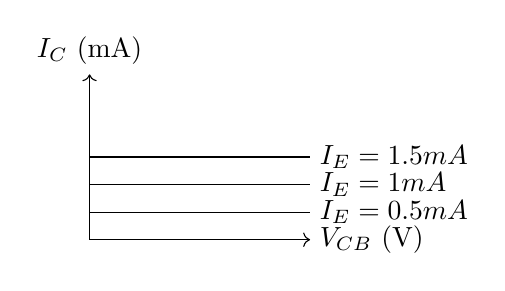
\begin{tikzpicture}[scale=0.7]
    \draw[->] (0,0) -- (4,0) node[right] {$V_{CB}$ (V)};
    \draw[->] (0,0) -- (0,3) node[above] {$I_C$ (mA)};
    
    % Curves
    \draw (0,0.5) -- (4,0.5) node[right] {$I_E=0.5mA$};
    \draw (0,1) -- (4,1) node[right] {$I_E=1mA$};
    \draw (0,1.5) -- (4,1.5) node[right] {$I_E=1.5mA$};
    
    % Active region mostly flat
\end{tikzpicture}
\captionof{figure}{Output Characteristics of CB Config}
\end{center}

\begin{itemize}
    \item \textbf{Active Region:} $I_C$ is almost independent of $V_{CB}$ and depends only on $I_E$. ($I_C \approx I_E$).
    \item \textbf{Saturation Region:} $V_{CB} < 0$. $I_C$ drops.
\end{itemize}
\end{solutionbox}

\end{document}




